\newpage
Here is an example of how to make images work in \LaTeX \\
% make it scale to something, and give the image, no need to specify path as we know to look into the folder images
\begin{figure}[h]
\centering % centre is you want
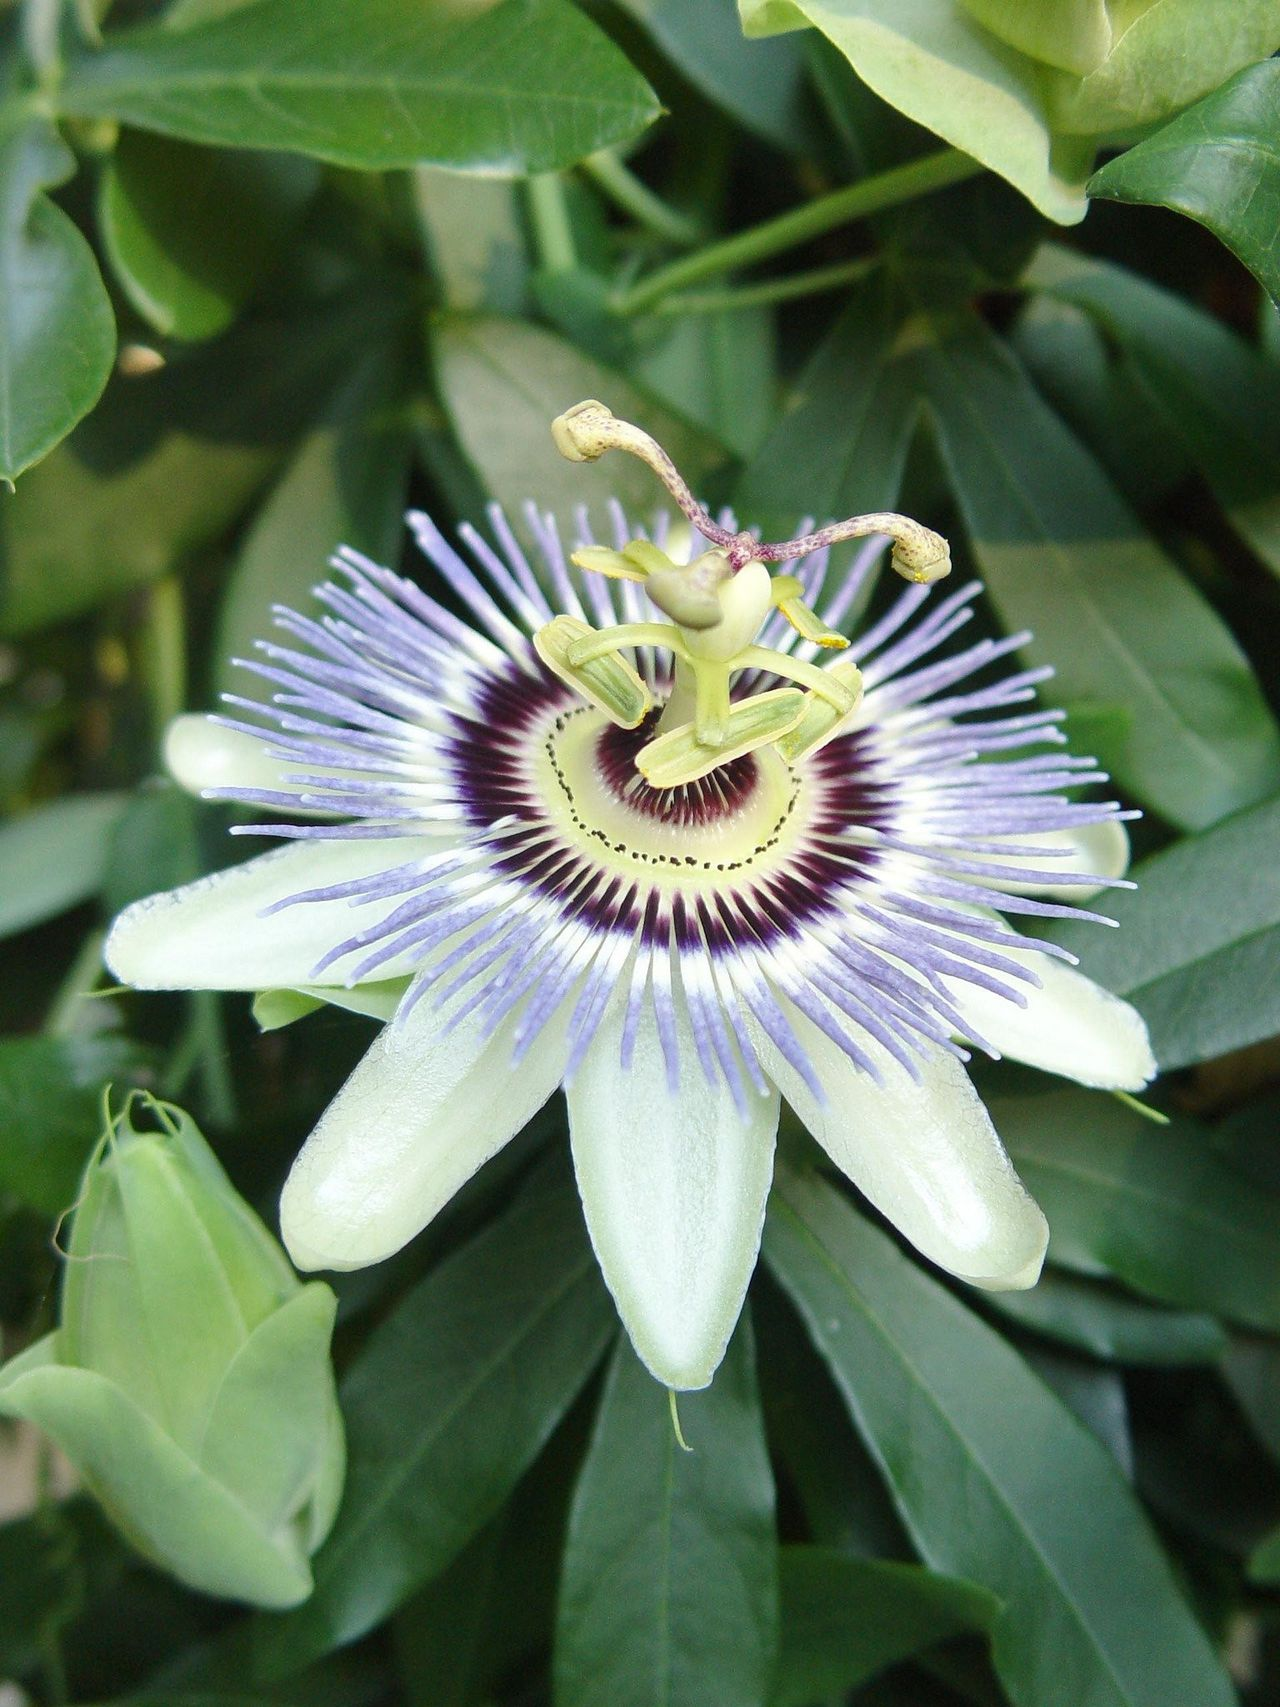
\includegraphics[scale=0.05]{example-flower} % To learn more go to: https://www.overleaf.com/learn/latex/Inserting_Images 
\caption{Example of the passion fruit flower}
\label{fig: passion-fruit-flower} % Can be used with function \ref{fig: passion-fruit-flower} to reference to image
\end{figure}
\\ % new line
The flower as shown in figure \ref{fig: passion-fruit-flower} is a beautiful flower.

\newpage
\section{Introduction} % title of section

% import .tex files from folder to keep things modular and short
\import{./SubSections/}{Overview-Purpose-of-System}
\import{./SubSections/}{Scope}
\import{./SubSections/}{Objectives-and-Success-Criteria}
\import{./SubSections/}{Definitions-and-Abbreviations}
\import{./SubSections/}{References}
%newpage % remove comment to create a newpage if needed (can be used in-between imports as well)
